Aplikacja webowa jest jedyną częścią systemu, do której użytkownik może mieć bezpośredni dostęp. Strona powstała w celu maksymalnego uproszczenia procesu badania kolejnych algorytmów i usług, które różniły się sposobem podawania danych wejściowych, sposobem uczenia oraz formatem zwracanych odpowiedzi. Do pozostałych zalet takiego rozwiązania należy ułatwienie przechowywania danych, poprzez umieszczenie ich we wspólnym miejscu co pomaga, w późniejszej interpretacji wyników.
\begin{figure}[H]
	\centering
	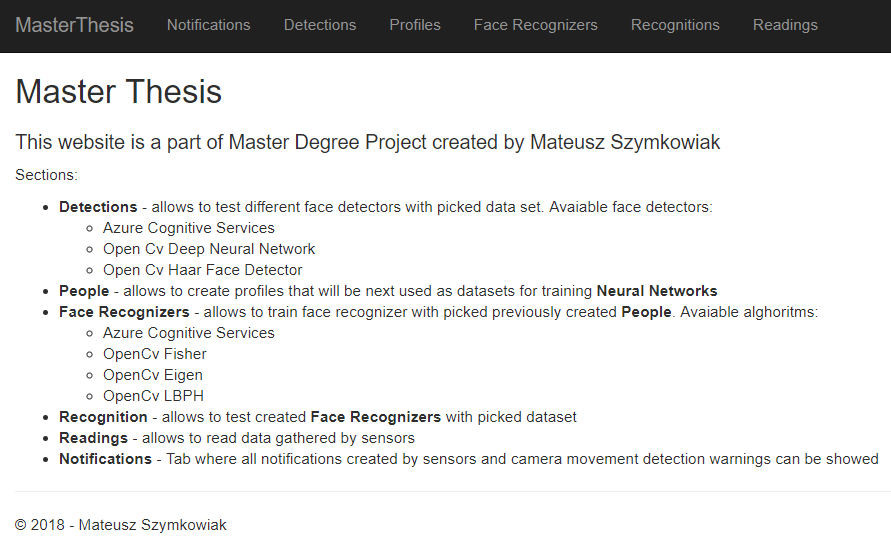
\includegraphics[scale=0.7]{aplikacja_webowa_razor_widok.png}
	\caption{Wygląd strony głównej}
	\label{fig:strona_glowna_razor}
\end{figure}
Zgodnie z interfejsem przedstawionym na rysunku \ref{fig:strona_glowna_razor}, strona została podzielona na 5 głównych sekcji:
\begin{itemize}
\item Detections- detekcje,
\item People- ludzie,
\item Neural Networks- sieci neuronowe,
\item Recognition- rozpoznawanie,
\item Sensor Readings- odczyty sensorów.
\end{itemize}

\section{Technologie}
Aplikacja webowa powstała w najnowszej kompilacji .NET Core 2, będącej międzyplatformową strukturą open source o wysokiej wydajności służącą do tworzenia nowoczesnych aplikacji internetowych opartych na usługach chmurowych. Logika biznesowa aplikacji została zaprogramowana w języku C\#. Warstwa widoku powstała w dwóch dostępnych rozwiązaniach, nieznacznie różniących się wyglądem, ale znacznie odbiegających od siebie sposobem działania. Przed omówieniem poszczególnych rozwiązań przedstawiono, krótkie definicje wykorzystanego wzorca projektowego MVC oraz technologii SPA. 

\subsection{Rozwiązanie 1- Razor Pages}
Pierwsza wersja została oparta o strony tworzone w technologi Razor Pages opartej o składnię Razor oraz podstawowe technologie webowe: HTML i CSS. Taki sposób tworzenia warstwy prezentacji jest zalecany dla aplikacji .NET Core, ponieważ pozwala zminimalizować ilość pracy wymaganej na jej utworzenie oraz zapewnia bardzo prosty proces wdrożenia. Aplikacja utworzona z pomocą Razor'a została zaprezentowana na rysunku \ref{fig:strona_glowna_razor}.

\subsection{Rozwiązanie 2- Angular 4}
Druga wersja widoku aplikacji oferuje dostęp do tych samych możliwości co pierwsze rozwiązanie, ale powstała przy pomocy frameworka webowego- Angular 4. Strona główna widoczna jest na rysunku \ref{fig:strona_glowna_angular}. Angular jest open sourcowym frameworkiem używanym do tworzenia aplikacji SPA (Single Page Application), napisany w języku TypeScript i wspierany oraz rozwijany przez Google.
\begin{figure}[H]
	\centering
	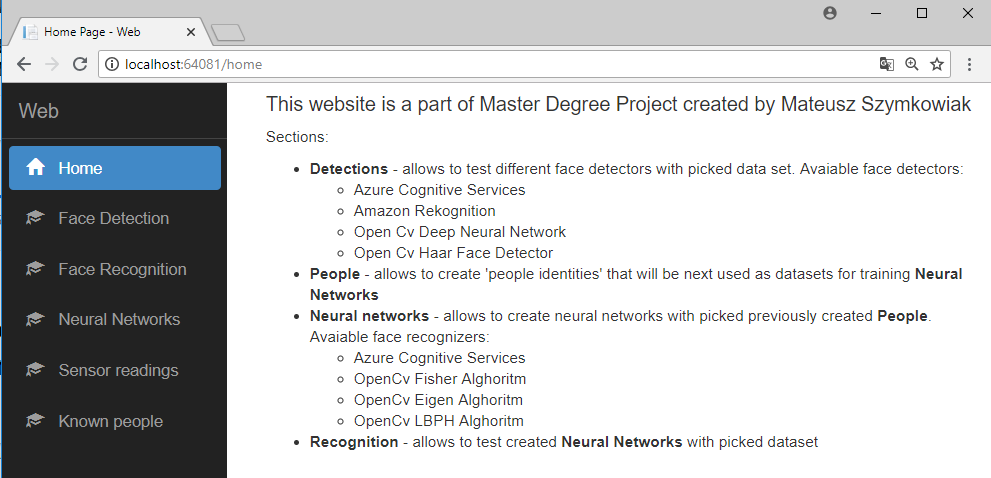
\includegraphics[scale=0.6]{aplikacja_webowa_angular_widok.png}
	\caption{Strona główna widoku utworzonym w Angular 4}
	\label{fig:strona_glowna_angular}
\end{figure}

\section{Detekcja twarzy}
Detections jest stroną odpowiedzialną za wykrywanie twarzy na obrazach przesłanych do systemu. Na głównej stronie możemy zobaczyć wszystkie zlecone detekcje, zarówno nowe jak i już zakończone.
\begin{figure}[H]
	\centering
	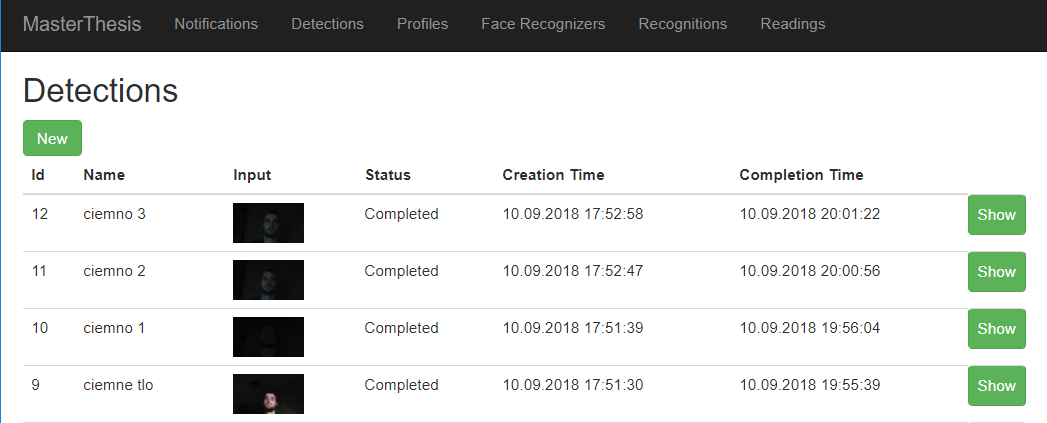
\includegraphics[scale=0.6]{detections.png}
	\caption{Widok detekcji twarzy}
	\label{fig:detections}
\end{figure}
Przycisk 'New' widoczny na \ref{fig:detections} pozwala na stworzenie nowego zadania wykrycia twarzy na obrazie, które zostanie przetworzone przez moduł aplikacji konsolowej. Na formularzu z rysunku \ref{fig:new_detection} należy podać nazwę zadania oraz za pomocą przycisku 'Wybierz plik' wybrać obraz w formacie png,jpg lub jpeg znajdujący się na dysku użytkownika.
\begin{figure}[H]
	\centering
	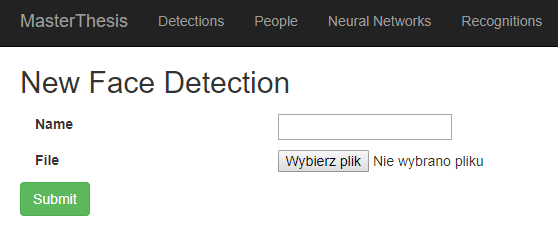
\includegraphics[scale=0.6]{new_detection.png}
	\caption{Tworzenie nowej detekcji}
	\label{fig:new_detection}
\end{figure}
Użycie przycisku 'Show' widocznego przy każdym zadaniu detekcji na rysunku \ref{fig:detections}, pozwoli na wyświetlenie szczegółów związanych z requestem, w tym wyników jeśli zadanie zostało zakończone.
\begin{figure}[H]
	\centering
	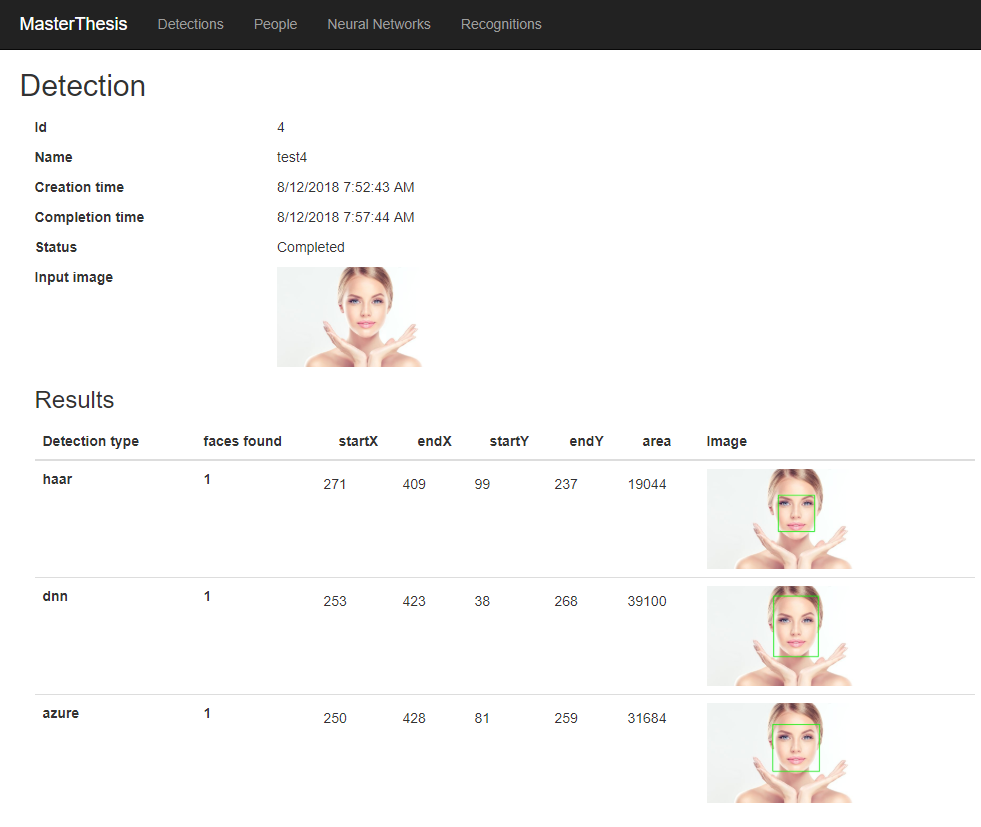
\includegraphics[scale=0.6]{detekcja_z_wynikami.png}
	\caption{Widok zakończonej detekcji}
	\label{fig:detekcja_zakonczona}
\end{figure}
Strona ze zdjęcia \ref{fig:detekcja_zakonczona} pozwala sprawdzić datę utworzenia oraz zakończenia zadania, obraz wejściowy, szczegółowe informacje o obszarze zidentyfikowanym jako twarz oraz sposobie jej wykrycia.
\section{Ludzie}
Strona 'People' służy do tworzenia nowych znanych tożsamości, które później mogą zostać wykorzystane jako dane uczące podczas trenowania sieci neuronowych. Do każdej osoby musi zostać przypisany zasób minimum 2 zdjęć. W przypadku braku możliwości wykrycia twarzy na zdjęciu, zostanie ono zignorowane podczas procesu nauczania.
\begin{figure}[H]
	\centering
	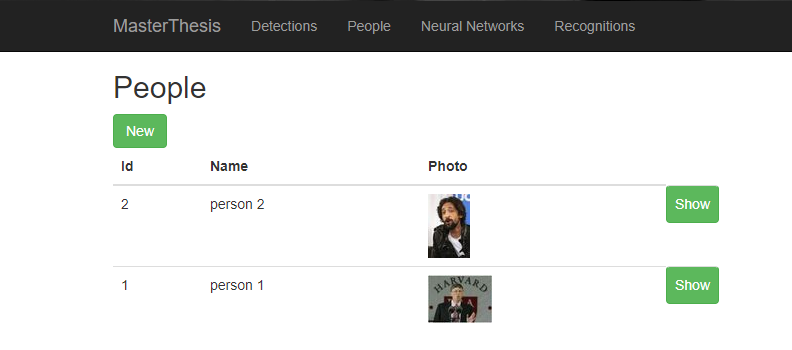
\includegraphics[scale=0.6]{people.png}
	\caption{Lista utworzonych ludzi}
	\label{fig:people}
\end{figure}
Nowa osoba może zostać utworzona w podobny sposób jak request detekcji twarzy. Jedyną różnicą jest wymóg wyboru kilku obrazów.
\begin{figure}[H]
	\centering
	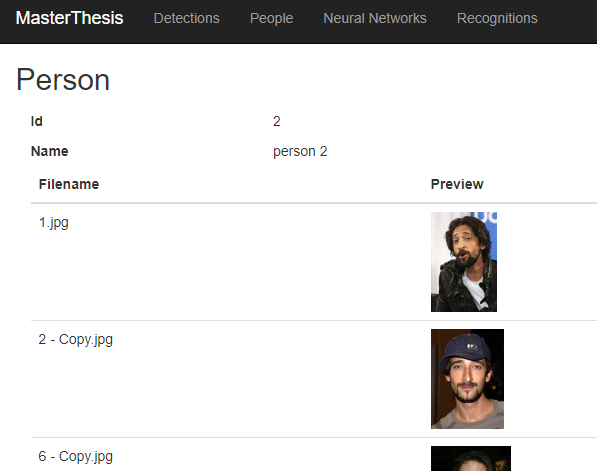
\includegraphics[scale=0.6]{person.png}
	\caption{Widok osoby}
	\label{fig:person}
\end{figure}
Utworzona osoba nie może być modyfikowana. Pierwsze załadowanie widoku osoby może trwać wydłużony czas z powodu procesu generowania linków do plików magazynowanych w usłudze Dropbox.

\section{Sieci neuronowe}
\begin{figure}[H]
	\centering
	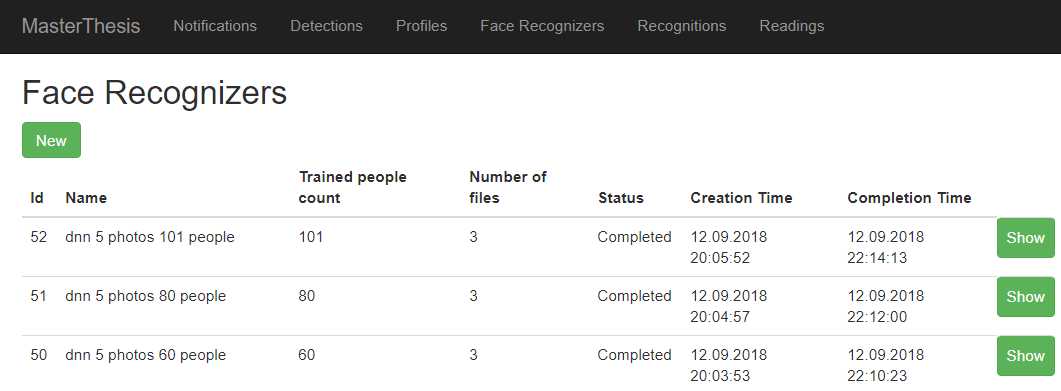
\includegraphics[scale=0.6]{neural_networks.png}
	\caption{Strona przedstawiająca istniejące grupy usług rozpoznawania tożsamości}
	\label{fig:sieci_neuronowe}
\end{figure}
W zakładce 'Neural Networks' użytkownik ma możliwość stworzenia grupy wybranych usług i sieci neuronowych, które zostaną nauczone rozpoznawać tożsamości utworzone w zakładce 'People'.
\begin{figure}[H]
	\centering
	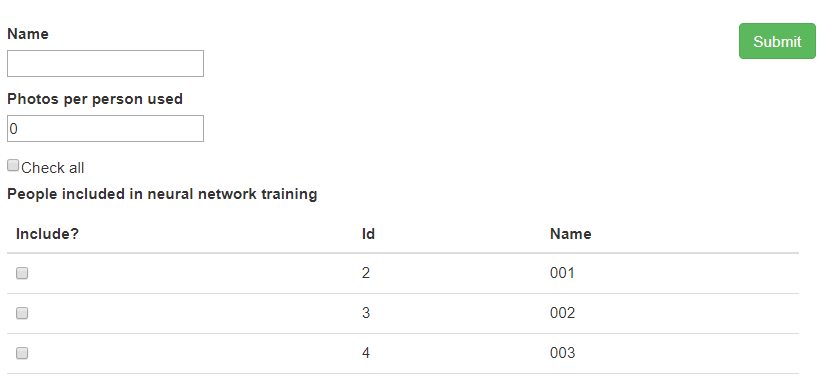
\includegraphics[scale=0.6]{nowa_siec.png}
	\caption{Tworzenie nowej grupy sieci neuronowych}
	\label{fig:nowa_siec}
\end{figure}
Każda istniejąca osoba zostanie wyświetlona jako checkbox, który należy zaznaczyć jeśli użytkownik chce by dana osoba została wykorzystana podczas procesu trenowania. Należy wybrać minimum 2 osoby, w przypadku wyboru mniejszej ilości osób, użytkownik zostanie poinformowany o tej konieczności.

Widok ukazany na rysunku \ref{fig:sieci_neuronowe} pozwala sprawdzić ile osób zostało użytych w procesie nauki oraz ile sieci neuronowych zostało utworzonych. Wyświetlenie jednej z grup pozwoli na uzyskanie bardziej szczegółowych informacji na temat wykorzystanych osób i utworzonych sieci, patrz rysunek \ref{fig:siec_neuronowa}.
\begin{figure}[H]
	\centering
	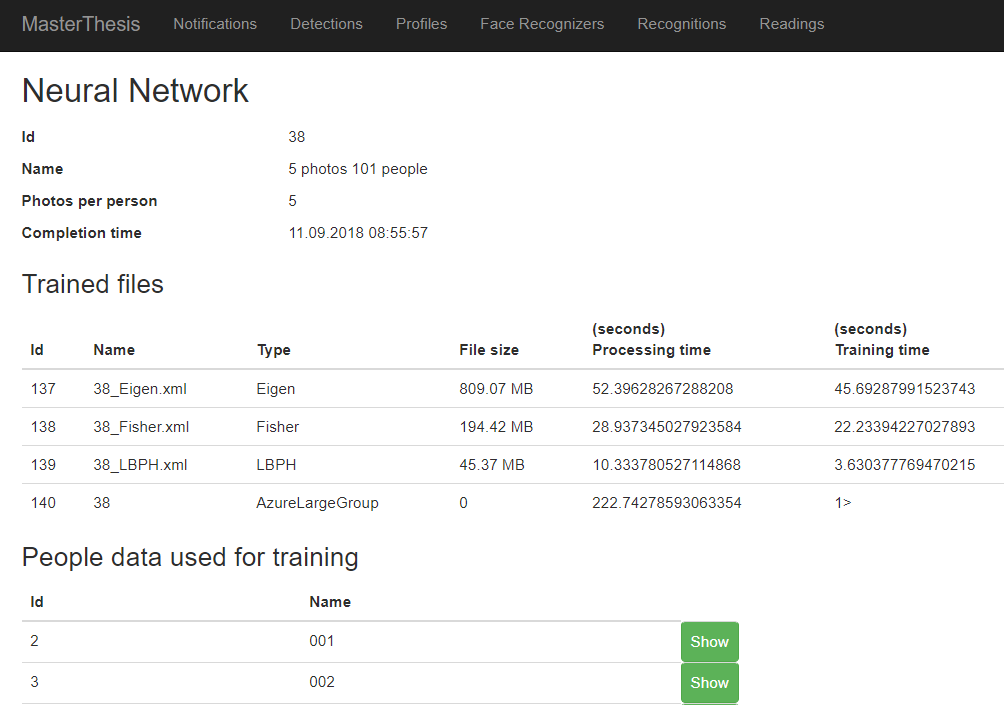
\includegraphics[scale=0.6]{siec_neuronowa.png}
	\caption{Szczegółowe informacje o grupie sieci neuronowych}
	\label{fig:siec_neuronowa}
\end{figure}

\section{Rozpoznawanie tożsamości}
W sekcji 'Recognitions' użytkownik ma możliwość wykorzystać wcześniej utworzone zbiory sieci neuronowych w celu identyfikacji tożsamości na zdjęciu przedstawiającym pojedynczą osobę.
\begin{figure}[H]
	\centering
	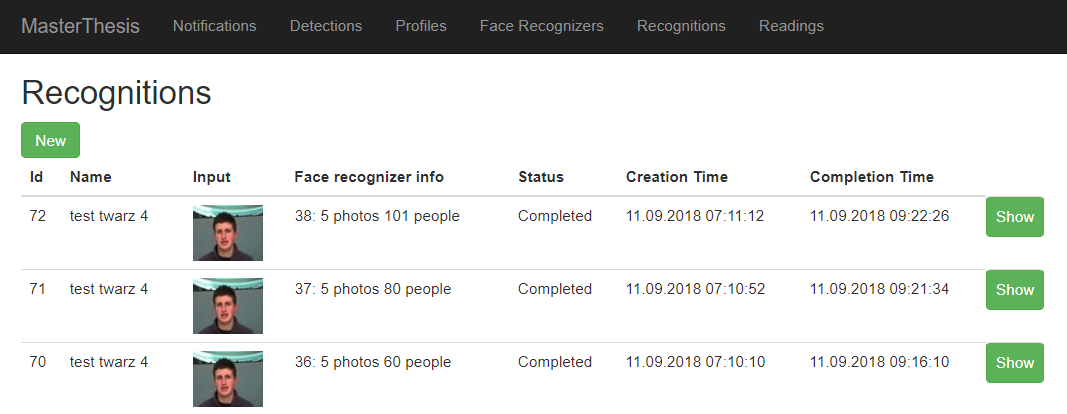
\includegraphics[scale=0.6]{recognitions.png}
	\caption{Lista zadań identyfikacji osoby}
	\label{fig:recognitions}
\end{figure}
Podobnie jak na pozostałych stronach, podczas tworzenia nowego zadania użytkownik będzie musiał uzupełnić prosty formularz. W formularzu przedstawionym na rysunku \ref{fig:new_recognition} należy załączyć jedno zdjęcie oraz wybrać grupę sieci neuronowych, która ma zostać wykorzystana do identyfikacji tożsamości osoby.
\begin{figure}[H]
	\centering
	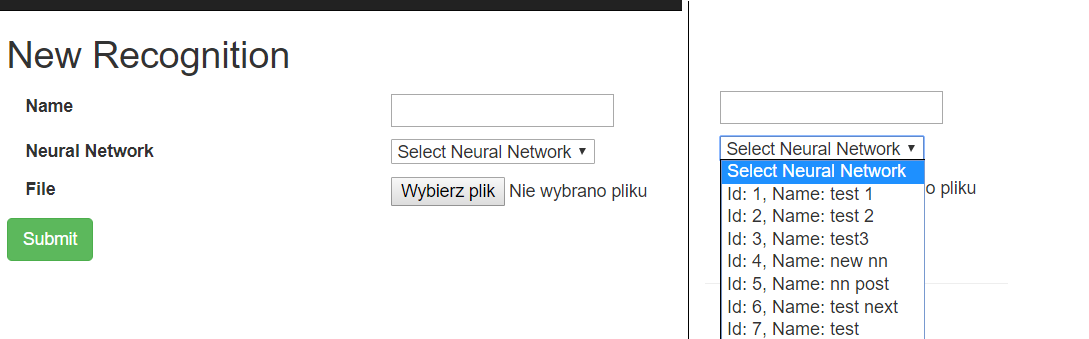
\includegraphics[scale=0.6]{new_recognition.png}
	\caption{Formularz tworzenia zadania identyfikacji}
	\label{fig:new_recognition}
\end{figure}
Po zakończonym procesie identyfikacji opisanym w kolejnym podrozdziale, użytkownik może wyświetlić wynik uzyskany przez każdą sieć dostępną w grupie. Przykładowy rezultat widoczny jest na zdjęciu \ref{fig:recognition}.
\begin{figure}[H]
	\centering
	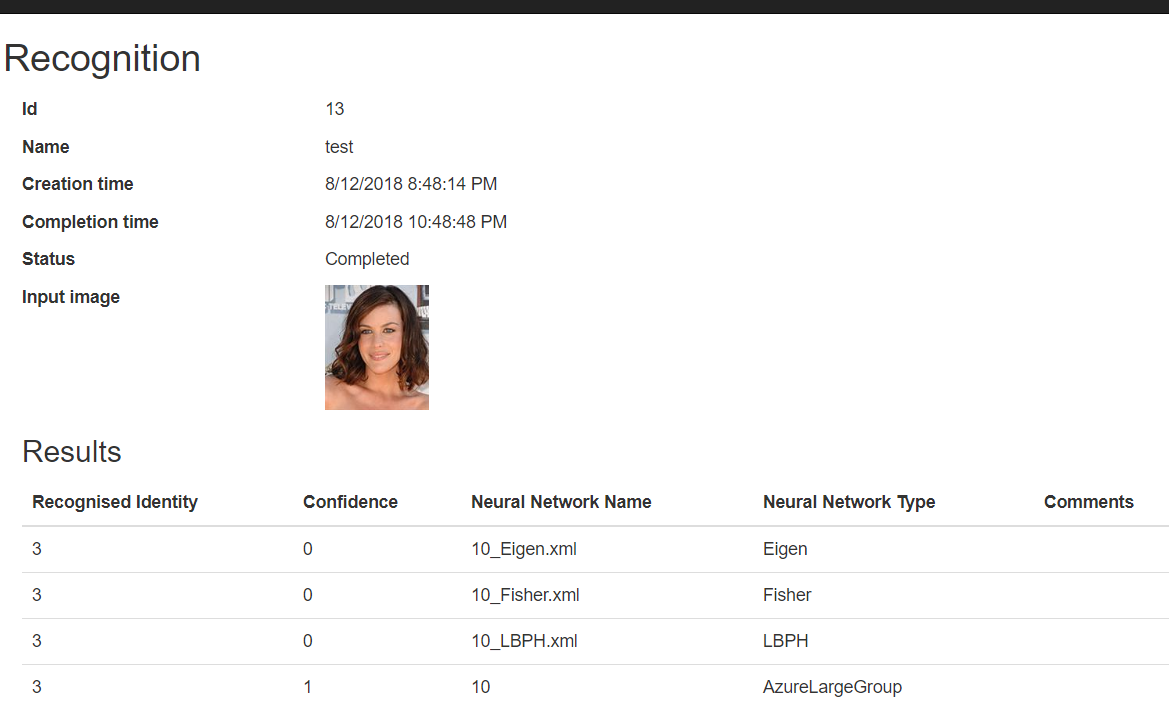
\includegraphics[scale=0.6]{recognition.png}
	\caption{Zakończony request identyfikacji}
	\label{fig:recognition}
\end{figure}

\section{Odczyty sensorów}
Zakładka Readings powstała w celu czytelnej prezentacji odczytów zebranych z sensorów w dniach funkcjonowania systemu. Odczyty zbierane są co minutę co generuje znaczną ilość wpisów do wyświetlenia. Z tego powodu po wejściu na stronę należy wybrać dzień, którym zainteresowany jest użytkownik. Przykładową listę zaprezentowano na rysunku \ref{fig:all_days}. Po wybraniu dnia ukazuje się widok, na którym przedstawiono wszystkie odczyty zebrane w wybranym okresie czasu.Do dostępnych informacji należą temperatura, wilgotność powietrza oraz czas wykonania pomiaru.
\begin{figure}[H]
	\centering
	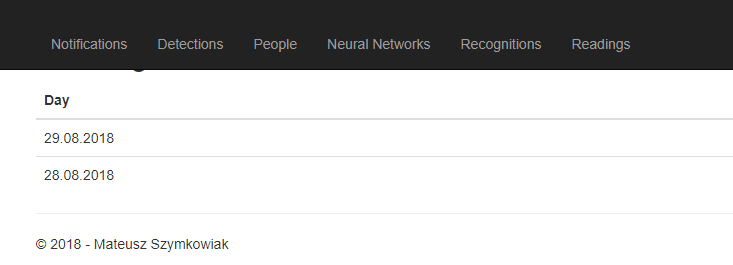
\includegraphics[scale=0.7]{all_days.png}
	\caption{Widok pozwalający na wybór dnia}
	\label{fig:all_days}
\end{figure}
\begin{figure}[H]
	\centering
	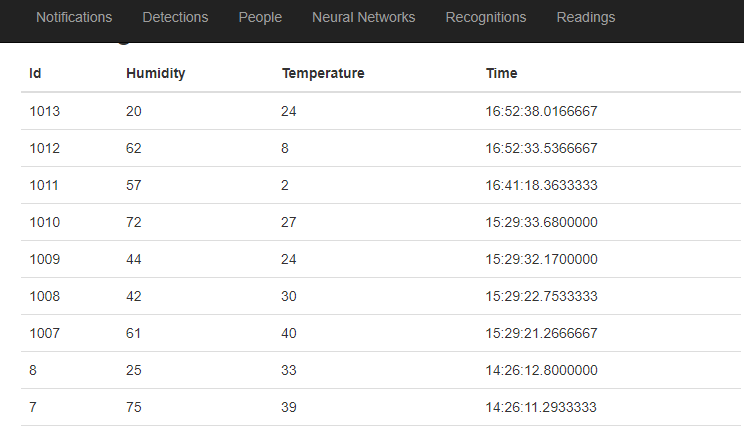
\includegraphics[scale=0.7]{daily_readings.png}
	\caption{Widok wyświetlający wszystkie odczyty z wybranego dnia}
	\label{fig:daily_readings}
\end{figure}

\section{Powiadomienia} \label{notifications}
Ostatnią ze stworzonych zakładek są Powiadomienia. Widok służy do wyświetlania wszystkich powiadomień utworzonych przez system, na które składają się:
\begin{itemize}
\item powiadomienia sensorów,
\item wykrycia ruchu.
\end{itemize}
 Typy oraz sposób ich generowania został szerzej opisany w rozdziale \ref{aplikacja_zarzadzanie}. Każde wyświetlane powiadomienie posiada wiadomość,typ oraz czas utworzenia. W przypadku wykrycia ruchu dodatkowo wyświetlone zostaje zdjęcie uchwyconego wydarzenia. Kilka przykładowych powiadomień można zaobserwować na rysunku \ref{fig:notifications}.
\begin{figure}[H]
	\centering
	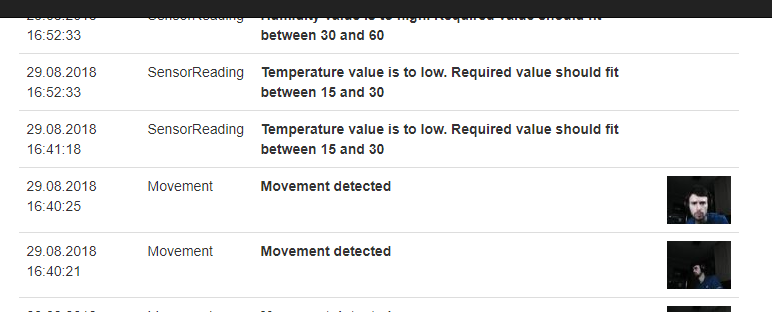
\includegraphics[scale=0.7]{notifications.png}
	\caption{Widok wyświetlający wszystkie odczyty z wybranego dnia}
	\label{fig:notifications}
\end{figure}